\chapter{Introducción}
\label{ch:intro}

La \acrfull{ai} como área de conocimiento ha experimentado un creciente interés en los últimos años. Esto no siempre ha sido así; desde su nacimiento ha ido alternando épocas de mucha actividad y de muy poca, debido a las altas expectativas que generan los nuevos avances en el área. Sin embargo, en la actualidad es muy difícil encontrar un campo que no se beneficie directamente de sus técnicas.

Una de las razones es su carácter multidisciplinar ya que, aunque pertenece al campo de la computación, es transversal a muchos otros campos de naturaleza muy diferente como, por ejemplo, la biología, la neurología o la psicología.

Dentro del área de la \ac{ai} es común diferenciar dos tipos de aproximaciones a la hora de representar el conocimiento: el enfoque \textbf{clásico}, que postula que el conocimiento como tal se puede reducir a un conjunto de símbolos con operadores para su manipulación, y el enfoque de la \acrfull{ci}, que defiende que el conocimiento se alcanza a través del aprendizaje, y que basa sus esfuerzos en la simulación de elementos de bajo nivel esperando que el conocimiento \enquote{emerja} de la interacción de éstos.

El límite entre ambos conjuntos no está perfectamente definido, más aún si tenemos en cuenta las diferentes terminologías existentes, las sinergias entre distintas técnicas dentro del área y los diferentes puntos de vista sobre éstas por parte de los autores. Sin embargo, una de las principales diferencias de ambos paradigmas es el punto de vista a la hora de solucionar problemas, siendo la aproximación \textbf{top-down} la usada en problemas de \acrshort{ai} clásica y la \textbf{bottom-up} la típica usada en la \acrshort{ci}. Revisaremos las diferencias entre conceptos de diferentes autores en el capítulo \nameref{ch:sota-ci}.

Uno de los campos de aplicación es el de los \gls{its}. Éstos se definen como un conjunto de aplicaciones orientadas a gestionar el transporte en todos sus aspectos (e.g. conducción eficiente, diseño de automóviles, gestión del tráfico o señalización en redes de carreteras) para hacerlos más eficientes y seguros. El interés es tal que en el año 2010 se publicó la directiva 2010/40/UE (ver \cite{parliament2010directive}) en la que se estableció el marco de implantación de los \ac{its} para toda la Unión Europea, quedando éstos definidos como:

\blockquote{[Los \ac{its} \ldots] son aplicaciones avanzadas que, sin incluir la inteligencia como tal, proporcionan servicios innovadores en relación con los diferentes modos de transporte y la gestión del tráfico y permiten a los distintos usuarios estar mejor informados y hacer un uso más seguro, más coordinado y «más inteligente» de las redes de transporte.}

La \textit{conducción} es una tarea muy compleja que involucra la ejecución de muchas tareas cognitivas pertenecientes a diversos niveles de abstracción. El concepto del \textit{tráfico} puede verse como un sistema complejo que emerge de las interacciones de agentes muy diversos, incluyendo a aquellos que realizan la tareas de conducir. El comportamiento durante la tarea de conducción es un objeto interesante de estudio: la evaluación de los conductores para conocer su manera de actuar en determinados escenarios nos permite, por ejemplo, detectar qué factores pueden afectar más o menos sobre determinados indicadores (e.g. el consumo estimado para una ruta en concreto). Sin embargo, la evaluación en algunos casos puede no ser posible debido a limitaciones como, por ejemplo, el tiempo, el dinero o la peligrosidad del escenario.

Los simuladores de tráfico son una solución para muchas de estas limitaciones, pero suelen basar su funcionamiento en modelos de conductor que responden a funciones más o menos complejas, alejadas de la realidad, además con pocas o ningunas opciones de personalización. Esto provoca que dichos modelos se adapten poco al comportamiento de un conductor en concreto.

Esta tesis pretende explotar la generación de modelos de conductor para simuladores que respondan al comportamiento de conductores reales usando, para ello, técnicas pertenecientes al campo de la \ac{ci}. Estos perfiles extraídos se aplicarán a un entorno de simulación basado en \acrfull{mas}. Así, una vez configurado el entorno, se podrán estudiar aspectos generales como la evolución del tráfico con determinados perfiles o particulares como el estilo de conducción o el impacto de los sistemas de asistencia.

\section{Motivación}

Los conceptos introducidos al comienzo del capítulo obedecen a una necesidad de la sociedad en la que vivimos, y que afecta tanto a nuestra generación como a las venideras: la eficiencia en el transporte. Dado que es imprescindible saber que existe un problema para arreglarlo, nada mejor que puntualizar algunos hechos de sobra conocidos:

\begin{itemize}
	\item En el año 2016, el número de vehículos a nivel mundial superó los $1.350$ millones, con una tendencia creciente \cite{oica2014motrate}. Reducir en un pequeño porcentaje el consumo evita la emisión de toneladas de gases considerados nocivos para el medio ambiente y el ser humano\footnote{Uno puede argumentar que el parque automovilístico se recicla con nuevos vehículos eléctricos categorizados \enquote{de consumo 0}. La triste realidad es que estos vehículos consumen la electricidad generada actualmente de una mayoría de centrales de combustibles fósiles y nucleares. Además, mientras que en países desarrollados el crecimiento ha sido en torno al 4-7\%, en países subdesarrollados, donde no existe aun infraestructura para la recarga de vehículos eléctricos, dicho crecimiento ha superado el 120\%.}.
	\item Aunque existen diferentes puntos de vista acerca de cuándo se agotarán las reservas de petróleo, los combustibles fósiles son recursos \textbf{finitos}. Lo más probable es que no se lleguen a agotar debido a la ley de la oferta y la demanda, pero hay que recordar que el petróleo se usa como base para la producción de otros muchos tipos de productos, como por ejemplo la vaselina, el asfalto o los plásticos.
	\item La emisión de gases está correlacionada con el aumento de la temperatura del planeta. Con el ritmo actual, dependiendo de la fuente estamos o bien llegando obien ya hemos sobrepasado un punto de no retorno con consecuencias catastróficas para la vida en el planeta.
	\item La conducción eficiente afecta directamente a factores correlacionados con el número de accidentes de tráfico. Un factor de sobra conocido es el de la velocidad, relacionado no sólo con el número sino con la gravedad de los accidentes (\cite{imprialou2016re}). Otros indicadores son las aceleraciones, deceleraciones y maniobras de cambio de dirección, cuyas frecuencias son directamente proporcionales a la agresividad, falta de seguridad y accidentes e inversamente proporcionales a la eficiencia (\cite{dingus2006100, lerner2010exploration}).
\end{itemize}

Éstos son sólo algunos hechos que ponen de manifiesto la necesidad de centrarse en el problema de cómo hacer de la conducción una actividad más eficiente y segura. Por ello, la \textbf{conducción eficiente} o \textit{eco-driving} se define como la aplicación de una serie de reglas de conducción con el objetivo de reducir el consumo de combustible, independientemente del tipo (e.g. electricidad, gasolina, \ldots).

Si es posible discriminar entre conductores eficientes y no eficientes se pueden identificar los hábitos recurrentes en estos últimos y adecuar la formación para eliminar dichos hábitos. Más aún teniendo en cuenta la relación existente entre la peligrosidad y algunas conductas agresivas. Un ejemplo donde la identificación de perfiles no eficientes pueden tener impacto claro económico y social es el de las empresas cuya actividad se basa en el transporte de mercancías o de personas.

Sin embargo, identificar la conducta de un conductor no es fácil, dado que su comportamiento se ve condicionado por numerosos factores como el estado de la ruta, el del tráfico o el estado físico o anímico. Además, la ambigüedad de las situaciones dificulta todavía más la identificación. Por ejemplo, un conductor puede ser clasificado en un momento como agresivo o no eficiente en una situación, únicamente porque su comportamiento ha sido condicionado por las malas reacciones de otros conductores conductores.

El análisis de todos los posibles casos es una tarea prácticamente imposible. Por ello, las simulaciones pueden dar una estimación de los posibles resultados de un estudio en el mundo real. Las simulaciones con \acrlongplsp{mas} representan a los conductores como agentes independientes, permitiendo la evaluación del comportamiento tanto individual como general del sistema en base a sus individuos a través de iteraciones discretas de tiempo.

Si el comportamiento de dichos agentes es extraído a partir de los datos reales de conductores, su comportamiento dentro de la simulación podría ser considerado como fuente de datos aproximada de comportamiento en situaciones de tráfico del mundo real. De esta forma, se dispondría de un marco de trabajo para la comparación de diferentes conductores sin necesidad de exponerlos a todos y cada uno de los posibles eventos posibles. También sería factible evaluar sistemas de asistencia evitando los problemas de no comparabilidad de condiciones del entorno entre pruebas.

Demostrar que la evaluación de un modelo del conductor en entornos simulados es equivalente a la evaluación de conductores en entornos reales implica que se pueden comparar dos conductores usando un criterio objetivo, es decir, sin depender del estado del resto de factores a la hora de realizar la prueba de campo. Dicho de otro modo, implicaría que es posible comparar la eficiencia de dos conductores independientemente del estado del tráfico e, incluso, sobre rutas diferentes.

\section{Objetivos}
\label{ch:intro:objectives}

El objetivo de esta tesis doctoral es la de demostrar las hipótesis~H\ref{hyp:first} y~H\ref{hyp:second}, quedando dicha demostración dentro de los límites impuestos por los supuestos y restricciones indicados más adelante.

\begin{hyp}[H\ref{hyp:first}] \label{hyp:first}
	La aplicación de técnicas pertenecientes al campo de la \ac{ci} sobre datosde conductores reales para la obtención de modelo de conducción permitirá incorporar características humanas no reproducibles por los modelos lineales existentes, mejorando la calidad de dichas simulaciones.
\end{hyp}

\begin{hyp}[H\ref{hyp:second}] \label{hyp:second}
	La aplicación de técnicas pertenecientes al campo de la \ac{ci} con datos extraídos de un entorno de microsimulación de espacio continuo y tiempo discreto basado en sistemas multiagentes permitirá modelar, de manera fiel a la realidad, el comportamiento de conductores reales.
\end{hyp}

Por tanto, el objetivo de la tesis es el de simular el comportamiento de conductores en entornos de micro-simulación a partir de su comportamiento en entornos reales usando técnicas de \ac{ci}. Para ello se consideran los siguientes objetivos específicos:

\begin{itemize}
	\item Estudiar y aplicar técnicas de la \ac{ci} sobre el área de la conducción.
	\item Realizar un estudio naturalista de conducción\sidenote{
		Un \textbf{estudio naturalista de conducción} basa su funcionamiento en la captura masiva de datos de conducción, normalmente involucrando una gran cantidad de sensores, para analizar el comportamiento del conductor, las características del vehículo, la vía, etcétera. La cantidad de sensores y la velocidad de captura hacen que la tarea de analizar y extraer conclusiones sea una tarea prácticamente imposible para un humano, por lo que es necesario el uso de técnicas de análisis de datos que suelen recaer en los campos de la estadística y del aprendizaje automático.
	} sobre conductores reales para:
	\begin{enumerate}
		\item Generar modelos personalizados de conductor a partir de los datos de conducción obtenidos.
		\item Aplicar modelos de conductores a entornos de simulación multiagente.
		\item Validar los modelos de conductor contra conductores reales.
	\end{enumerate}
	\item Estudiar la efectividad de sistemas de asistencia encaminados a mejorar la eficiencia y analizar el comportamiento de conductor.
\end{itemize}

\subsection{Supuestos}

\begin{itemize}
	\item La circulación se supone por la derecha de la vía en el sentido de la circulación, siendo los carriles de lento a rápido de derecha a izquierda respectivamente.
	\item Los datos de los que extraer el comportamiento se corresponderán con lecturas realizadas durante el día, con buena visibilidad y sin lluvia.
	\item El tipo de vehículo sobre el que modelar el comportamiento será el \textit{utilitario}.
	\item El conductor a modelar pertenecerá al grupo más representativo de conductores. Esto se corresponde con varón de $35$ a $39$ años (ver figura~\ref{fig:drivers-ages-per-genre}).
\end{itemize}

\begin{figure}[t]
	\centering
	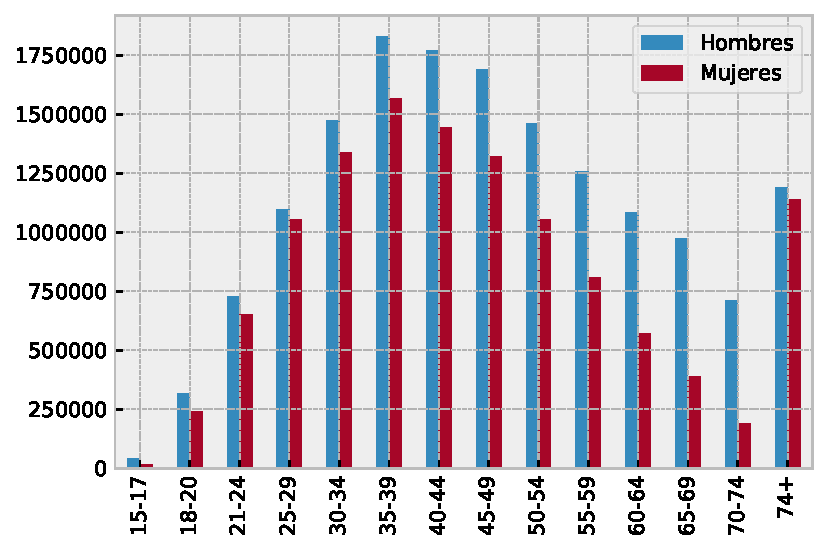
\includegraphics[width=.8\textwidth]{drivers-ages-per-genre}
	\caption[Censo de conductores según género y edad]{Último censo de conductores según género segmentado por edades. Fuente: Dirección General de Tráfico (\url{dgt.es}).}
	\label{fig:drivers-ages-per-genre}
\end{figure}
\subsection{Restricciones}

\begin{itemize}
	\item Los modelos generados se corresponderán a entornos urbanos.
	\item Reduciremos el comportamiento del conductor a los de circulación en línea y en cambio de carril\sidenote{
		Son conocidos en la literatura como modelos de \textbf{aceleración} y modelos de \textbf{cambio de carril}. Entraremos en detalle sobre ambos conceptos en el capítulo~\nameref{ch:sota-behavior-models}.
	}.
	\item La resolución máxima del modelo creado será de \SI{10}{\hertz}.
	\item En el caso de los modelos que hacen uso de \acrlongplsp{ann}, no se pueden explicar las razones del comportamiento inferido.
\end{itemize}

\section{Estructura de la tesis}
\label{ch:intro:structure}


La tesis se divide en tres partes. La primera se corresponde con el estado de la cuestión, compuesta por los capítulos \nameref{ch:sota-ci}, \nameref{ch:sota-traffic-simulation} y \nameref{ch:sota-behavior-models}, explicando en qué punto se encuentra la literatura de los temas en los que se apoya la presente tesis.

En la segunda parte se desarrolla el tema del modelado de conductores: En \nameref{ch:methodology} se describe la adquisición y tratamiento de datos, junto con algunas de las decisiones tomadas durante el proceso; después, en \nameref{ch:longitudinal-model} y \nameref{ch:lane-change-model} se desarrollan los procesos de obtención de los modelos longitudinal y de cambio de carril respectivamente. En \nameref{ch:specific-models} se extiende el proceso entrenamiento a conductores en particular y en \nameref{ch:simulation-implementation}, se introducen los comportamientos de los modelos de conductor implementados en un simulador.

Por último, se expondrán las \nameref{ch:conclusions} junto con una serie de posibles \nameref{ch:future-work} consideradas interesantes tras la realización de la tesis.
